\chapter{Bài toán tìm kiếm}

%%%%%
\section{Mở đầu}

Thông thường, một vài vấn đề thực tế có điểm bắt đầu và điểm kết thúc, hay còn gọi là đáp án của vấn đề đó. Thế nhưng ta không có một thuật toán hay gì mà ta có thể thực hiện theo và tìm được đáp án, do đó ta cần \textbf{tìm kiếm} đáp án cho vấn đề đó \cite{GraphSearch}. Thế nhưng điều kiện tiên quyết để giải quyết bài toán tìm kiếm đó, ta cần biểu diễn được nó \cite{LHB}.
\vspace{7pt}

Ta có thể biểu diễn một \textbf{bài toán tìm kiếm} thông qua năm thành phần chính, để giải quyết tốt hơn, ta đưa bài toán tìm kiếm thành 1 đồ thị:
\begin{itemize}
    \item \textbf{Không gian trạng thái}: Bao gồm tất cả các trạng thái có thể có của bài toán. Trạng thái trong bài toán tìm kiếm là thể hiện của một giai đoạn trong quá trình giải bài toán tìm kiếm, một trạng thái sẽ bao gồm những thông tin về môi trường xung quanh bài toán tìm kiếm \cite{LHB}. Ta xem 1 trạng thái như là 1 nút của đồ thị, do đó cả không gian trạng thái là cả 1 đồ thị.

    \item \textbf{Trạng thái bắt đầu}: Là nơi bắt đầu của bài toán hay là nơi bắt đầu việc tìm kiếm của ta.

    \item \textbf{Trạng thái kết thúc}: Là nơi mà bài toán kết thúc, hay ta có thể nói là đích đến của ta khi thực hiện việc tìm kiếm, lúc này ta sẽ tìm được ``đáp án'' cho bài toán. Giống như thực tế, đôi khi đích đến không chỉ một mà ta còn có thể nhiều đích đến, do đó trạng thái kết thúc có thể là một trạng thái hoặc là một tập hợp các trạng thái. Ngoài ra trạng thái kết thúc có thể được biểu diễn bằng một điều kiện nào đó chứ không còn là một trạng thái xác định nữa \cite{LHB}.

    \item \textbf{Hàm chuyển trạng thái con}: Là một hàm nhận trạng thái hiện tại và cho ra tất cả các trạng thái mà trạng thái hiện tại có thể di chuyển đến được. Ta có thể xem hàm chuyển trạng thái con này như là một cạnh giữa hai nút trong đồ thị với mỗi nút tương ứng với một trạng thái.

    \item \textbf{Hàm chi phí}: Hàm này cho ta biết việc chuyển giữa một trạng thái này sang trạng thái khác sẽ tốn chi phí như thế nào. Ta có thể xem hàm chi phí như là một trọng số của cạnh của đồ thị.
\end{itemize}

Giờ ta đã có thể biểu diễn được một bài toán tìm kiếm rồi, tiếp theo ta chỉ cần \textit{tìm kiếm} được đáp án. Thế nhưng ta sẽ tìm kiếm như thế nào ? Ta xét một đồ thị là không gian các trạng thái, bắt đầu tại một nút trên đồ thị, xem đó là trạng thái bắt đầu. Ta tạo hai danh sách gọi là $frontier$ và $expanded$. Trong đó $frontier$ sẽ chứa danh sách những nút mà ta đã tìm thấy và ``chuẩn bị'' đi đến, ta gọi những nút đó là \textit{discovered node} (hay \textit{nút đã khám phá}), còn $expanded$ sẽ chứa những nút mà ta đã đi đến và tìm tất cả những nút tiếp theo mà ta có thể đi đến được, ta gọi những nút đó là \textit{expanded node}. Còn những nút còn lại, ta sẽ gọi là \textit{unexplored node}. Nguyên lý là ta đi đến nút nào, gọi nút đó là \textit{current node}, ta sẽ mở rộng nút đó, thêm $current$ vào $expanded$ và thêm các nút được mở rộng vào $frontier$ nếu nó chưa nằm trong $frontier$ và $expanded$, sau đó ta lấy các nút trong $frontier$ làm $current$, mở rộng tiếp tục cho đến khi \textit{current node} của ta là trạng thái đích hoặc nếu $frontier$ đã hết nút, ta sẽ trả về không có đáp án.

\begin{figure}[H]
    \centering
    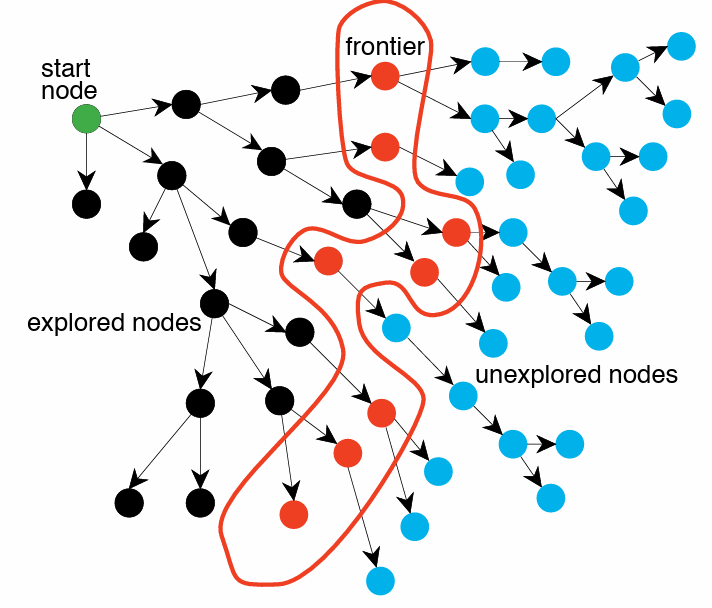
\includegraphics[scale=0.7]{figure/illustration.png}
    \caption{Minh hoạ cho nguyên lý của cách giải một bài toán tìm kiếm. Nguồn \cite{GraphSearch}.}
    \label{fig:illu}
\end{figure}

Dưới đây là mã giả cho cách giải tổng quát một bài toán tìm kiếm thông qua đồ thị:
\vspace{10pt}

\begin{algorithm}[H]
  $start \gets \text{trạng thái bắt đầu}$\;
  $frontier \gets \{start\}$\;
  $expanded \gets \emptyset$\;
  $goal \gets \text{hàm xem nút hiện tại có là trạng thái đích hay chưa}$\;
  $T \gets \text{hàm chuyển trạng thái con}$\;
  \While{$frontier \neq \emptyset$}
  {
      $current \gets \text{nút được lấy ra từ $frontier$}$\;
      \text{Thêm $current$ vào $expanded$}\;
      \eIf{$goal(current)$}
      {
        \KwRet{\text{đã tìm thấy đáp án}}\;
      }{
        \For{$neighbor \in T(current)$}
        {
            \If{$neighbor \notin frontier$ và $neighbor \notin expanded$} 
            {
                \text{Thêm $neigbor$ vào $frontier$}\;
            }
        }
      }
  }
  \KwRet{\text{không tìm thấy đáp án}}\;
  \caption{Tìm kiếm đồ thị}
  \label{algo:1}
\end{algorithm}

%%%%%
\section{Các định nghĩa cơ bản}

\begin{defivn} \textbf{Hệ số phân nhánh tiến} (\textit{forward branching factor}) của một nút là số lượng cạnh đi ra từ nút đó.
\end{defivn}

\begin{defivn} \textbf{Hệ số phân nhánh lùi} (\textit{backward branching factor}) của một nút là số lượng cạnh đi vào (đi đến) nút đó.
\end{defivn}

\begin{defivn} Một thuật toán tìm kiếm được nói là có \textbf{tính đầy đủ} (\textit{completeness}) nếu tồn tại ít nhất một đáp án thì thuật toán tìm kiếm của ta đảm bảo sẽ tìm được đáp án đó. Để có tính đầy đủ, một thuật toán tìm kiếm phải \textbf{có tính hệ thống} (\textit{systematic}), nghĩa là nó có thể đi đến được mọi trạng thái mà đi được từ trạng thái ban đầu.
\end{defivn}

\begin{defivn} Một thuật toán tìm kiếm được nói là có \textbf{tính tối ưu} (\textit{optimality}) nếu nó có thể tìm được đáp án có chi phí thấp nhất trong tất cả các đáp án.
\end{defivn}

\begin{defivn} \textbf{Độ phức tạp thời gian} (\textit{time complexity}) của một thuật toán tìm kiếm là thời gian của thuật toán chạy và được biểu diễn bằng độ dài đường đi dài nhất $m$ và hệ số phân nhánh lớn nhất $b$.
\end{defivn}

\begin{defivn} \textbf{Độ phức tạp không gian} (\textit{space complexity}) của một thuật toán tìm kiếm là bộ nhớ mà thuật toán dùng và được biểu diễn bằng $m$ và $b$.
\end{defivn}

%%%%%
\section{Tìm kiếm không thông tin và tìm kiếm có thông tin}

\textbf{Tìm kiếm không thông tin} (\textit{Uninformed Search}) là tìm kiếm mà ngoài việc biết được trạng thái đích là gì thì thuật toán không còn thông tin gì khác, ví dụ như trạng thái hiện tại có gần trạng thái đích hay không ? Ngoài ra tìm kiếm không thông tin còn được gọi là \textit{tìm kiếm mù} do ta không biết thông tin gì khác về trạng thái đích ngoài việc trạng thái đích trong như thế nào.
\vspace{7pt}

Khác với bên trên \textbf{tìm kiếm có thông tin} (\textit{Informed Search}) hay còn gọi là \textit{tìm kiếm Heuristic}, sẽ có thêm thông tin để biết được mình đã gần trạng thái đích hay chưa, thông tin này ở dạng hàm, được gọi là \textbf{hàm heuristic}, kí hiệu là $h(n)$:
$$
h(n) = \hspace{3pt} \text{ước lượng chi phí của đường đi ngắn nhất từ $n$ đến trạng thái đích}
$$
thông thường, các chi phí, ta gọi là $g(n)$, là tổng các trọng số từ trạng thái bắt đầu đến nút $n$. Thế nhưng nếu chi phí là bằng nhau, thì ta sẽ chọn đi đến nút kế tiếp như nào, lúc đấy $h(n)$ sẽ giúp ta chọn nút đi đến kế tiếp, $h(n)$ có thể được xem như là \textit{knowledge} của thuật toán tìm kiếm.

\begin{defivn}
    Ta gọi một hàm heuristic $h(n)$ là \textbf{chấp nhận được} (\textit{admissible}) nếu nó không \textit{ước lượng quá cao} chi phí từ $n$ đến trạng thái đích, nghĩa là:
    $$
    0 \leq h(n) \leq h^*(n)
    $$
    với $h^*(n)$ là chi phí tối ưu thật sự từ $n$ đến trạng thái đích.
\end{defivn}

\begin{defivn}
    Ta gọi một hàm heuristic $h(n)$ là \textbf{nhất quán} (\textit{consistent}) nếu với mọi nút $n$ và mọi nút con $n'$ của nó, ta có:
    $$
    h(n) \leq cost(n, n') + h(n')
    $$
    trong đó $cost(n, n')$ là chi phí để đi từ $n$ đến $n'$. Ngoài ra, mọi hàm heuristic $h(n)$ nếu nhất quán thì chấp nhận được, ngược lại thì không. Do đó nhất quán là một điều kiện chặn hơn của chấp nhận được.
\end{defivn}

\begin{figure}[H]
    \centering
    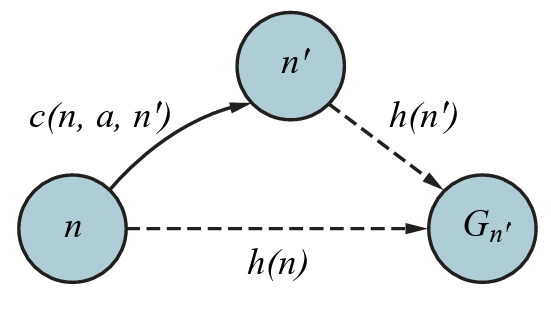
\includegraphics[scale=0.65]{figure/consistent.png}
    \caption{ Ta có thể thấy định nghĩa $8$ giống như \textbf{bất đẳng thức tam giác}, hình \ref{fig:consistent} được lấy từ \cite{Russell_Norvig_Chang_2022}, trong đó $c(n, a, n')$ là chi phí đi từ $n$ đến $n'$ thông qua hành động $a$.}
    \label{fig:consistent}
\end{figure}

Ta có thể thấy điểm khác nhau đầu tiên giữa tìm kiếm có thông và không có thông tin là tìm kiếm có thông tin có thêm hàm heuristic $h(n)$ để định hướng cho nó, việc này giúp nó tìm được đích nhanh hơn tìm kiếm không thông tin do không đi những đường đi có chi phí cao, hoặc đi những đường đi có khả năng không dẫn tới đích, ngoài ra nó cũng không phải đi hết tất cả các trạng thái để tìm được trạng thái đích. Do đó, tìm kiếm có thông tin sẽ có thể tìm được các đường đi có chi phí thấp nhất, vì vậy khả năng tối ưu của nó cao hơn tìm kiếm không có thông tin.
\vspace{7pt}

Thế nhưng, tìm kiếm không thông tin sẽ dễ dàng cài đặt hơn do ta không cần quan tâm đến các chi phí hay việc chọn hàm heuristic của tìm kiếm có thông tin. Tiếp theo tìm kiếm không thông tin là có hệ thống khi nó luôn đi đến mọi trạng thái từ trạng thái ban đầu, nhờ vậy, các thuật toán tìm kiếm không tin dễ dàng có tính đầy đủ hơn.
\vspace{7pt}

Và điều quan trọng nhất, ta cần biết bài toán nào nên áp dụng phương pháp tìm kiếm nào, trong các bài toán có không gian trạng thái quá lớn, tìm kiếm không thông tin sẽ mất thời gian rất lâu do phải đi hết (hoặc gần hết) các trạng thái, trong các bài toán không quá phức tạp, tìm kiếm không thông tin lại tốt hơn do dễ dàng cài đặt.
\vspace{7pt}

Các thuật toán thuộc tìm kiếm không có thông tin có thể kể đến như Breadth-First-Search, Depth-First-Search, Uniform-Cost-Search và tìm kiếm có thông tin như Greedy Best-First-Search, $\text{A}^*$ Search.